\chapter{Methodology}\label{Method}
In this chapter, we will cover several methods which construct the outline of the thesis. Thus, we will be able to look at the localization problem from different perspectives. The main idea of this chapter is understanding the technical background and manipulating them in a way that gathering plausible information out of different sensors.
%-------------------Odometry------------------------------%
%---------------------------------------------------------%
\section{Odometry}\label{sec:odom}
To estimate a position of mobile robots there are two basic approaches are used: \textit{absolute} and \textit{relative positioning}. For calculating relative positioning, the odometry is used i.e, observing wheel revolutions over the time to compute traveled distance from a known starting point \cite{odometry1}. Indeed, odometry result is unreliable in a long-term due to the unbounded accumulation of error, although odometry is accepted as an essential method for robot navigation by researchers because of its attributes such as being inexpensive, straightforward and easing the fundamental problem of position determination \cite{odometry2}. 
\\
\par Odometry employs simple geometric equations to find the displacement of the robot as follows:
\begin{equation}
    c_m = \pi D_n/nC_e \\
\end{equation}
\begin{equation}
    \Delta X_{L/R,i} = c_mN_{L/R,i} 
\end{equation}
where: \\
\begin{tabular}{l l}
    $c_m$ &:coefficient that converts pulses into linear wheel displacement; \\
    $D_n$ &:wheel diameter (in mm); \\
    $n$ &:gear ratio;\\
    $C_e$ &:encoder resolution;\\
    $N_{L/R}$ &:pulse increment left and right respectively;\\
    $\Delta X_{L/R}$ &:traveled distance left and right respectively.
\end{tabular}
\\
\\
Here, rest of the well-known odometry equation is left over to Appendix for being expressed in more detail.
\\ 
\par Odometry relies on above expressed equations which are easy to apply in real time on robots. However, odometry is subject to two different errors as stated in Borenstein J. et al. \cite{odometry1} which are \textit{systematic} and \textit{non-systematic error}:
\begin{table}[h!]
\renewcommand{\arraystretch}{2}
    \centering
    \begin{tabular}{| l | l |}
    \hline
        1)Systematic Errors:            &2)Non-Systematic Errors:\\
    \hline
        unequal wheel diameters;        &travel over uneven grounds;\\
        misalignment of wheels;         &travel over unexpected objects;\\
        limited encoder sampling rate;  &wheel-slippage\\
    \hline
    \end{tabular}
\caption{Odometry Errors}
\label{lab:Odom_error}
\end{table}
\\
\par Due to the above reasons, odometry data are not eligible to be used for long-term localization and its results were investigated in chapter \textbf{\ref{sec:result}} for proving this argument.
%-------------------EKF------------------------------%
%---------------------------------------------------------%
\newpage
\section{Extended Kalman Filter}\label{ekf}
As mentioned in \cite{noise}, none of the sensors are perfect due to the conversion of the signal from analog to digital, therefore, sensor data are generally prone to noise. For that reason, the imperfectness should be eliminated, i.e, the noise part of the raw data must be filtered before proceeding any further application. To do it, the best approach is Kalman filter which is introduced by Kalman R.E. (1960) \cite{kalman}. Kalman Filter is a state estimator that curtails estimated error when the requirements converge to each other \cite{kalman1}. In this chapter well-known Kalman filter algorithm is not derived. However, its algorithm can be found in \cite{kalman}, \cite{kalman1} or \cite{kalman2}.
\\ 
\par Even though Kalman filter is a very powerful method for estimating state, it is only defined for linear systems. Hence, Kalman filter assumes a Gaussian distribution which means Gaussian signals can keep its attribute after passing through the linear system. However, if the system is non-linear, Gaussian distribution may not be Gaussian again as shown in Figure \ref{fig:Gaussion}.
\begin{figure}[h!]
    \centering
    \begin{subfigure}{.5\textheight}
        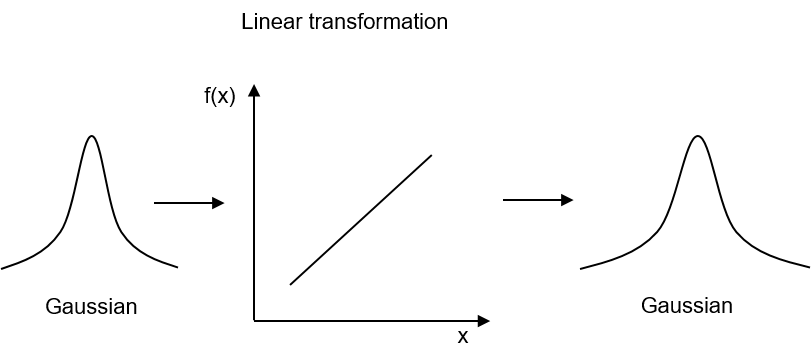
\includegraphics[scale=0.9]{linear.png}
        \label{fig:linear}
    \end{subfigure}
    \begin{subfigure}{.5\textheight}
        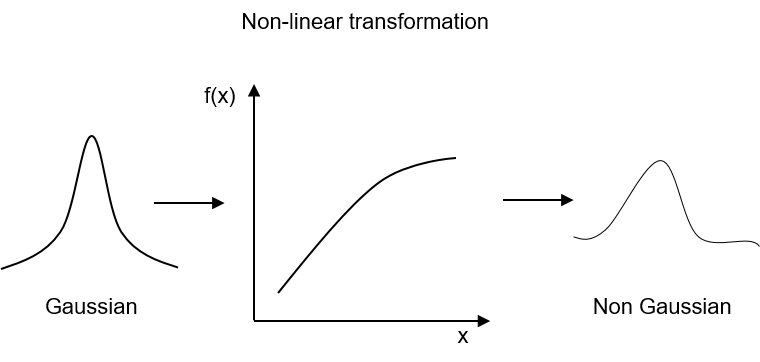
\includegraphics[scale=0.9]{non_liner.png}
        \label{fig:non-linear}
    \end{subfigure}
    \caption{Illustration of Gaussian over linear and non-linear system}
    \label{fig:Gaussion}

\end{figure}
\\
\par Nonetheless, from the mathematical point of view, the non-linear function can be linearized by using Taylor series expression %todo can be excluded.
that is presented by  Brook Taylor in 1715. 
Thus Kalman filter can be applied for non-linear systems as well and it is referred as \textit{extended} Kalman Filter or EKF. Let us look at the linearization of non-linear system and set of EKF equations \cite{kalman3}.

\begin{wrapfigure}[15]{l}{0.4\textwidth}
  \begin{center}
    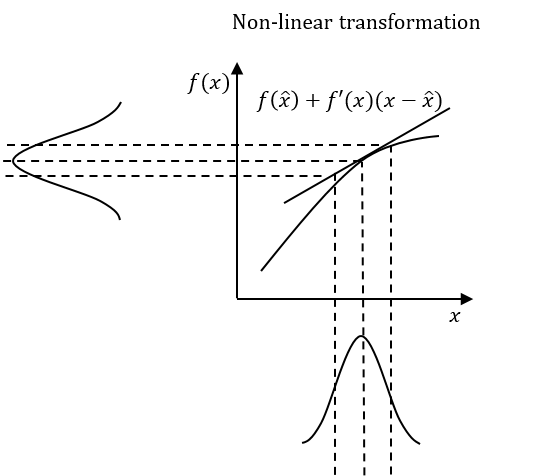
\includegraphics[width=0.4\textwidth]{linearization}
  \end{center}
  \caption{Linearization}
  \label{fig:linearization}
\end{wrapfigure}
\hspace{-13pt}System:
\vspace{-33pt}
\begin{eqnarray}\label{eq:non_linear}
    x_k=f(x_k,u_k)+w_k\\
    z_k=h(x_k)+v_k  \label{eq:non_linear1} 
\end{eqnarray}
\vspace{-13pt}
Jacobian:
\vspace{-20pt}
\begin{eqnarray}\label{eq:jacobian}
F=\frac{\partial f}{\partial x}|_{x_{k-1},u_k}\\
H=\frac{\partial h}{\partial x}|_{x_k}\label{eq:jacobian1}    
\end{eqnarray}
\vspace{-20pt}
Linearized:
\vspace{-20pt}
\begin{eqnarray}\label{eq:linearized}
\Delta x_k \approx F\Delta x_{k-1} + w_k\\
\Delta z_k \approx H\Delta x_{k} + v_k\label{eq:linearized1}
\end{eqnarray}
\\
\\
\begin{table}[h]
\renewcommand{\arraystretch}{2}
    \centering
    \begin{tabular}{| c | c |}
    \hline
        \textbf{a)EKF time update equations}            &\textbf{b)EKF measurement update equations}\\
    \hline
         $x_k^-=f(\hat x_{k-1},u_k,0)$        &$\hat x_k= \hat x_k^-+K_k(z_k-h(\hat x_k^-,0))$\\
          $P_k^-=A_kP_{k-1}A_k^T+W_kQ_{k-1}W_k^T$        &$K_k=P_k^-H_k^T(H_kP_k^-H_k^T+V_kR_kV_k^T)^{-1}$\\ 
          &$P_k=(I-K_kH_k)P_k^-$\\
    \hline
    \end{tabular}
\caption{EKF equations}%todo add nice name
\label{tab:ekf_eq}
\end{table}
\par In equation \eqref{eq:non_linear} and \eqref{eq:non_linear1}, the non-linear system and and its observation model with noise are described as a difference equation. Then, in following equations \eqref{eq:jacobian} and \eqref{eq:jacobian1}, the non-linear function and its observation model are linearized by taking derivative in respect of $x$ and they are stated in equation \eqref{eq:linearized} \eqref{eq:linearized1} respectively.
\\ After the non-linear system is approximated by linearization, EKF is a good option for state estimation. Apart from its advantages, we also need to mention the disadvantages of EKF. Hesam Khazraj et al. refer to some of the drawbacks of EKF in their study \cite{kalman5}. For instance, EKF is applicable as long as the higher order terms of the system are differentiable. Addition to this, calculating the Jacobian matrix is complicated and highly time-consuming.
\\ In following, we describe how it is implemented in the system in general \cite{kalman4}.  

\subsection*{Implementation}
As a first step, one model is created for states that to be estimated as in the following equation:
\begin{equation}
     x_k = Ax_{k-1}+Bu_k+w_{k-1}
\end{equation}
where $x_k$ is the states of interest, $u_k$ is well-known control signal and $w_k$ is normal distributed process noise with co-variance \textbf{Q}. $A$ is the state transition matrix whereas $B$ is the control matrix. As a remark that the control signal $u_k$ was not used in sense of this project. As a second step is defining observation model as following:
\begin{equation}
    z_k = Hx_k+v_k
\end{equation}
where $z_k$ is the observation vector at time k, $H$ is the measurement matrix and $v_k$ is the normal distributed measurement noise with co-variance \textbf{P}.
\\ 
\par Ultimately, Kalman filter will find to correct estimation of states by calculating Time Update and Measurement Update as formulated in table \textbf{\ref{tab:ekf_eq}}. It is important to note that EKF can achieve better estimation as long as noise parameters $w_{k-1}$, $v_k$ and their co-variance \textbf{Q} and \textbf{P} approximated well. 
\\ To conclude, we use EKF which is introduces by Thomas Moore et al. \cite{kalman4} in scope of thesis. The main reason that we use EKF is exploiting all sensors on a system without dealing with different measurement time, delay or etc\cite{kalman6}. In other words, we must be able to acquire plausible information from sensors even if the absence of any sensors at any time.
%-------------------NDT------------------------------%
%---------------------------------------------------------%
\newpage
\section{Normal Distribution Transform}\label{sec:ndt}
This section elaborates the \textit{normal distribution transform} (NDT) which was introduced by Biber et al. \cite{2dndt} and its extended version to 3D by Magnusson et al. \cite{3dndt}  for scan registration. It refers to find affine transformation between two consecutive laser scan. In robotic fields, it is commonly used method for providing accurate estimation of the odometry.%todo add reference and it is not common way actually it is relatively new
\\
\par The mainspring of NDT is describing a surface of a model by modeling the probability of finding a point at a certain position by means of the linear combination of normal distributions (see \cite{2dndt}, \cite{3dndt}), i.e, NDT breaks model point clouds into cells, which can be imaged a square in 2D or a box in 3D, and assigns a probability distribution to each cell. Thus NDT provides piece-wise representation about a surface of a model which means it is eligible to be applied optimization algorithm such as Newton optimization algorithm.
%TODO oku thesis localization
As mentioned before, the first step of the algorithm is breaking the space, that is occupied with points, into cells. Then, calculating the mean $\vec \mu$ of the point in the cell  and its co-variance matrix \textbf{C} for every single cell b as follows\cite{2dndt}:
\begin{align}
    \vec \mu &= \frac{1}{n}\sum_{k=1}^n \vec x_k\\
    C &=\frac{1}{1-n}\sum_{k=1}^n(\vec{x_k}-\vec{q})(\vec{x_k} -\vec{q})^T
\end{align}
where $\vec x_k=1,2,3,...,n$ are the points are kept in the cell. \\

\par The second step is modeling a probability that there is point at a certain position $\vec x$ in cell \textbf{b} by means of normal distribution and in following equation the probability density function is described \cite{3dndt}:
\begin{equation}
p(\vec x)=\frac{1}{2}exp(-\frac{(\vec{x}-\vec{\mu})^T\textbf{C}^{-1}(\vec{x}-\vec{\mu})}{2}),
\end{equation}
$\vec{p}$ is a vector that contains parameters to be optimized e.g. translation and rotation of the current pose. Let assume $\vec p=[\vec t | \vec r | \vec \phi ]$ where $\vec{t}=[t_x t_y t_z]$ is a translation, $\vec{r}=[r_x r_y r_z]$ is a rotation and $\phi$ is rotation angle. Furthermore, transformation matrix can be described by using $\vec{p}$, $\vec{x}$ and right-handed coordinate in 3D as follows \cite{3dndt}:
\begin{equation}
T(\vec{p},\vec{x})=
\begin{bmatrix}
tr_x^2+c		&tr_xr_y-sr_z	&tr_xr_z+sr_y\\
tr_xr_y+sr_z	&tr_y^2+c		&tr_yr_z-sr_x\\
tr_xr_z-s		&tr_yr_z+sr_x	&tr_z^2+c
\end{bmatrix}\vec{x}+ 
\begin{bmatrix}
t_x\\
t_y\\
t_z
\end{bmatrix}
\end{equation}
where t is 1-cos$\phi$, c is cos$\phi$ and s is sin$\phi$.
\\
\par Next step is measuring the fitness of transformation between reference and target scan by evaluating of the sum of PDFs whose value is called as score $s(p)$ in equation \ref{eq:score}. Afterward, the fitness score is optimized until converge to the required threshold by using the Newton optimization algorithm in equation \ref{eq:newton_opt} unless the fitness score is good enough as defined \cite{3dndt}:
\begin{equation}\label{eq:score}
    s(\vec p)=-\sum_{k=1}^np(T(\vec{p},\vec{x}))
\end{equation}
\begin{equation}\label{eq:newton_opt}
    \textbf{H}\Delta p =-g
\end{equation}
where \textbf{H} and $\vec{g}$ are the Hessian Matrix and gradient of s. Eventually, $\Delta p$ is added to the current pose in every iteration, $\vec p \xleftarrow[]{} \vec p+\Delta p$.

\subsection*{Cell size}
Since NDT represents the space with cells which are called voxel, the size of it has a great impact on the running time and accuracy of NDT. The consequence of selecting voxel size either too big or too small cause the object in scan be more blur, increasing the running time respectively. In section \ref{sec:result}, how the voxel size influence NDT algorithm is discussed.
%TODO:ADD ADVANTAGE AND DISADVANTAGE
%-------------------ICP------------------------------%
%---------------------------------------------------------%
\newpage
\section{Iterative Closest Point}\label{icp}
\textit{Iterative closest point}(ICP) is widely used for scan registration since it was presented by Besl et al. in 1992 \cite{icp}. ICP is employed to approximate the path of the car by sequentially search the common points in two sets point in a pair-wise manner. 
%todo expalin why we used it for localization
The key idea of ICP is that if the initial transformation is known between the reference and the target scan, the rest of correct transformation in terms of rotation matrix \textit{\textbf{R}} and translation vector \textit{\textbf{t}}, can be calculated in closed form \cite{icp1}, i.e., ICP finds the best match by utilizing the relationship between two corresponding points of two scans e.g. in equation \eqref{eq:icp_error}, minimizing the sum of squared distance between two matching point in two set of points denoting as $M=\{m_1,\dots,m_{N_m}\}$  and $D=\{d_1,\dots,d_{N_d}\}$ \cite{icp4}:
\begin{align}\label{eq:icp_error}
    E(R,t)&=\sum_{i=1}^{N_m}\sum_{j=1}^{N_d}w_{i,j} ||m_i -(Rd_j+t)||^2,
    \\
    w_{i,j}&=\begin{cases}
    1, &\text{if $m_i-T*dj \leq d_{max}$}\\
    0, &\text{else}
\end{cases}%todo explain weighting 
\end{align}
where $d_{max}$ is maximum matching threshold and $w$ is weight of the pairs. The reason behind of weighting the pairs depending on $d_{max}$ is preventing misalignment and rejecting some outlier pairs as show in Figure \ref{fig:icp}. 
\begin{figure}[h!]
  \centering
  \begin{tabular}{c c}
  \setlength{\fboxsep}{0pt}%
\setlength{\fboxrule}{1pt}%
\fbox{
    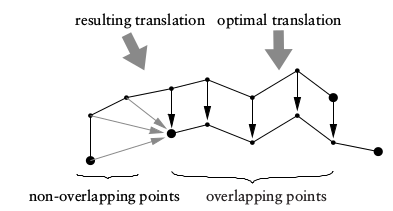
\includegraphics[scale=0.65]{icp_error.png}} & \rotatebox{90}{\footnotesize \textbf{Source}: Martin Magnusson \cite{icp2}}
  \end{tabular}
  \captionsetup{justification=justified,singlelinecheck=false}
  \caption{It illustrates incomplete overlap of two scan. In Figure, normal black arrows indicates corresponding point pairs whereas gray arrows indicate multi correspondences which must be eliminated for good matching.}
  \label{fig:icp}
\end{figure}
To do so, we decrease the execution time and increasing the accuracy of matching. However, this is not always the case as stated in Magnusson study \cite{icp2} that choosing small $d_{max}$ can make ICP more susceptible. Please also keep in mind that there is always a trade-off between time and accuracy by choosing $d_{max}$ \cite{icp3}. As a conclusion, ICP can briefly be summarized as follows:
\begin{itemize}
    \item Determining the corresponding points in two scan
    \item Calculating rotation matrix R and translation vector t
    \item Applying transformation to the points which is registered
    \item Iterate until fulfill the requirement
\end{itemize}

%-------------------Summary------------------------------%
%---------------------------------------------------------%
\section{Summary}\label{sec:summary}
To sum up everything, we studied related technical background in terms of implementation, advantages, and disadvantages. In the odometry part, we utilize the wheel encoder as the main sensor for estimating and tracking the position of the car. In the following section, we employed the EKF to facilitate synchronization of sensors such as IMU, wheel odometry, GPS etc. and estimate the future state of the position. In the last two section, we handled the term of scan registration in two different perspectives. Firstly, we studied NDT which is signifying the most probable points in the space as part of the surface. In contrast, ICP is representing the surface of a model by using every single point in the space. %todo deduction